% ACM AI Letters — 8-page paper
% PRM-Guided Cost-Aware Routing for Heterogeneous Agentic Pipelines
\documentclass[sigconf,natbib=false]{acmart}

\usepackage{booktabs}
\usepackage{multirow}
\usepackage{microtype}
\usepackage{graphicx}
\usepackage{amsmath}
\usepackage{xspace}
\usepackage{enumitem}
\usepackage[capitalize]{cleveref}

\newcommand{\prm}{\textsc{prm}\xspace}
\newcommand{\versa}{VersaPRM\xspace}
\newcommand{\proposed}{PRM-Guided\xspace}

\setcopyright{acmlicensed}
\copyrightyear{2026}
\acmYear{2026}
\acmDOI{}
\acmConference[ACM AI Letters '26]{}{}{}
\acmISBN{}

\begin{document}

\title{PRM-Guided Cost-Aware Routing for Heterogeneous Agentic Pipelines}

\author{Ansuman Nayak}
\affiliation{
  \institution{Georgia Institute of Technology}
  \city{Atlanta} \state{GA} \country{USA}}
\email{anayak306@gatech.edu}

\begin{abstract}
Enterprise agentic pipelines chain multiple LLM calls across heterogeneous step
types---retrieval, tool use, synthesis---where failure modes and compute costs
differ per step.  Current routing methods either route at query level
pre-execution or learn offline trajectory boundaries with no runtime process
signal.  We study whether multi-domain Process Reward Models (PRMs) can serve
as live step-quality routing signals across heterogeneous agent steps, and
whether PRM-conditioned three-tier routing improves the cost--accuracy tradeoff
beyond TRIM-style binary PRM routing and BAAR-style learned boundary routing.

On 1,000 AgentProcessBench trajectories (8,509 human-labeled steps), we find:
(1) VersaPRM is the only publicly available PRM with reliable cross-step-type
signal (Spearman $= +0.166$); math-specialist PRMs produce inverted signal on
retrieval steps.  (2) Three-tier PRM-guided routing strictly dominates TRIM at
every point in a 46-point Pareto sweep: $+10$ pp accuracy at matched cost,
$21$--$26\%$ cost reduction at matched accuracy.  (3) Routing transfers to
unseen banking/airline tasks with $10\%$ relative degradation vs.\ $16\%$ for
Uniform.  (4) Including retrieved context in PRM scoring yields the largest
single routing improvement ($+6.6$ pp)---larger than any routing policy change.
\end{abstract}

\keywords{agentic pipelines, routing, process reward models, cost-efficiency,
LLM inference}

\maketitle

% ─────────────────────────────────────────────────────────────────────────────
\section{Introduction}
% ─────────────────────────────────────────────────────────────────────────────

JPMorgan has deployed over 450 agentic AI workflows, with more than 230,000
employees interacting daily~\cite{jpmorgan2026}.  A typical enterprise pipeline
strings together retrieval, API calls, document parsing, reasoning, and
compliance checks.  Each step type has a distinct failure mode and a different
compute cost profile.  Routing each step to an appropriately sized model could
substantially reduce cost with minimal accuracy loss---but existing routing
methods are inadequate for this heterogeneous setting.

\textbf{Query-level routing} (FrugalGPT~\cite{frugalgpt2023},
DAAO~\cite{daao2025}) decides the model tier once, before execution, based on
estimated input difficulty.  This misses within-trajectory quality variation
and degenerates when difficulty proxies fail.  \textbf{Offline boundary routing}
(BAAR~\cite{baar2026}) learns step-routing boundaries from trajectory data
without any runtime process signal---it cannot adapt to failure patterns that
differ from training distribution.  \textbf{PRM-based routing} (TRIM~\cite{trim2026})
uses a Process Reward Model score to route between cheap and frontier models,
but only in homogeneous math chain-of-thought where every step is the same
type.

This paper combines the TRIM signal with the BAAR heterogeneous setting and
asks: \emph{do multi-domain PRMs provide reliable step-quality routing signals
across heterogeneous tool-using agent steps, and does PRM-conditioned routing
improve the cost--accuracy frontier?}

\paragraph{Contributions.}
\begin{enumerate}[leftmargin=*,topsep=2pt,itemsep=2pt]
  \item \textbf{Exp 1 (PRM signal evaluation).} We benchmark four PRMs as
    routing signals on 8,509 human-labeled agent steps and quantify the
    math-PRM transfer gap: Qwen2.5-Math-PRM achieves Spearman $= -0.036$
    (inverted); VersaPRM achieves $+0.166$, the only reliable signal.
  \item \textbf{Exp 2 (routing comparison).} A three-tier PRM-Guided router
    strictly dominates TRIM-style binary routing on a 46-point Pareto sweep:
    $+10$ pp accuracy at equal cost, $21$--$26\%$ cost reduction at equal
    accuracy.  BAAR over-escalates at $65\%$ to Tier 3, incurring higher cost
    than Frontier at lower accuracy than Uniform.
  \item \textbf{Exp 3 (PRM ablation).} Routing precision correlates with Exp~1
    signal quality; VersaPRM is the only PRM above the random escalation
    baseline (precision $0.536$ vs.\ $0.465$).
  \item \textbf{Exp 4 (generalization).} Zero-shot transfer to tau2 (banking/
    airline tasks) degrades PRM-Guided by only $10\%$ relative vs.\ $16\%$
    for Uniform.
  \item \textbf{Exp 10 (retrieval context).} Including retrieved passages in
    PRM scoring yields $+6.6$ pp routing accuracy---the largest improvement in
    the study, orthogonal to routing policy.
\end{enumerate}

% ─────────────────────────────────────────────────────────────────────────────
\section{Related Work}
% ─────────────────────────────────────────────────────────────────────────────

\paragraph{LLM routing and cascades.}
FrugalGPT~\cite{frugalgpt2023} cascades queries through models by estimated
cost-quality tradeoffs.  DAAO~\cite{daao2025} extends this to agentic
workflows, routing entire trajectories based on pre-execution difficulty
estimation.  BAAR~\cite{baar2026} learns step-level routing boundaries from
annotated trajectories, targeting the heterogeneous agent pipeline setting
without any process signal.

\paragraph{Process Reward Models.}
Math PRMs~\cite{lightman2023} score intermediate reasoning steps in
chain-of-thought.  Qwen2.5-Math-PRM~\cite{qwenprm2025} achieves state-of-the-art
on ProcessBench but is trained exclusively on mathematical reasoning.
VersaPRM~\cite{versaprm2025} extends multi-domain coverage via synthetic MMLU-Pro
training.  AgentRM~\cite{agentrm2025} targets web/shop/navigation environments
for test-time search reranking.  DG-PRM~\cite{dgprm2025} constructs dynamic
reward criteria via LLM judgment.  None of these have been used as runtime
routing signals for heterogeneous pipelines.

\paragraph{TRIM.}
TRIM~\cite{trim2026} uses PRM scores to switch between cheap and frontier
models in multi-step math reasoning, achieving $5$--$6\times$ cost reduction
in the homogeneous setting.  Our work extends this to heterogeneous pipelines
and three-tier routing.

\paragraph{Prompt compression.}
Caveman-style compression~\cite{jiang2023} and LLMLingua~\cite{llmlingua2023}
reduce prompt length before LLM calls.  Our Exp~9 and 10 are the first to
apply input compression specifically within a PRM-routing pipeline.

% ─────────────────────────────────────────────────────────────────────────────
\section{Method}
\label{sec:method}
% ─────────────────────────────────────────────────────────────────────────────

\subsection{System Overview}

\cref{fig:system} shows the full pipeline.  Three components work in sequence
for each agent step.

\textbf{(1) PRM Step Scorer.}  After step $t$ completes, VersaPRM scores the
step output on a $[0,1]$ quality scale:
\begin{equation}
  s_t = \text{VersaPRM}(\text{query} \| \text{retrieval\_ctx} \| \text{step\_text}_t)
\end{equation}
The inclusion of retrieval context (tool result passages) is motivated by Exp~10
(\S\ref{sec:exp10}).  Without it, VersaPRM cannot assess whether a retrieval step
returned relevant documents.

\textbf{(2) Routing Controller.}  A lightweight deterministic policy maps $s_t$
to a tier choice for step $t{+}1$:
\begin{equation}
  \text{tier}_{t+1} = \begin{cases}
    1 & s_t > \theta_h \\
    2 & \theta_l < s_t \leq \theta_h \\
    3 & s_t \leq \theta_l
  \end{cases}
\end{equation}
where $\theta_h$ and $\theta_l$ are calibrated to the 75th and 25th percentiles
of VersaPRM's score distribution on training trajectories ($\theta_h = 0.86$,
$\theta_l = 0.62$), ensuring a ${\approx}25\%/50\%/25\%$ tier split.

\textbf{(3) Pipeline Integration.}  A thin LangGraph wrapper intercepts
between steps, calls the scorer, and dispatches to the selected model tier.

\subsection{Model Tiers and Cost Model}

\begin{table}[h]
\small
\centering
\caption{Model tier definitions.}
\label{tab:tiers}
\begin{tabular}{llrrr}
\toprule
Tier & Model & \$/1M tok & $p_\text{good}$ & $p_\text{bad}$ \\
\midrule
1 & Llama-3.1-8B  & 0.20 & 0.92 & 0.30 \\
2 & Llama-3.1-70B & 0.90 & 0.97 & 0.65 \\
3 & Qwen2.5-72B   & 1.80 & 0.99 & 0.85 \\
\bottomrule
\end{tabular}
\end{table}

Outcome probabilities $p_\text{good}$ and $p_\text{bad}$ (\cref{tab:tiers})
define the counterfactual simulation: a step labelled good (human label $= +1$)
succeeds with $p_\text{good}(k)$ under tier $k$; a bad step ($= -1$) recovers
with $p_\text{bad}(k)$.  Task accuracy equals the product of per-step success
probabilities.

\subsection{Baselines}

We compare against seven methods:
\textbf{Always-Cheap} (Tier 1 always),
\textbf{Uniform} (Tier 2 always, primary baseline),
\textbf{Always-Frontier} (Tier 3 always, accuracy upper bound),
\textbf{DAAO}~\cite{daao2025} (question-length difficulty heuristic, pre-execution),
\textbf{BAAR}~\cite{baar2026} (logistic regression on step features, fitted on 800 train trajectories),
\textbf{TRIM-style}~\cite{trim2026} (binary T1/T3 PRM threshold), and
\textbf{Rule-based PRM} (fixed threshold, no Tier 2).

\begin{figure}[t]
  \centering
  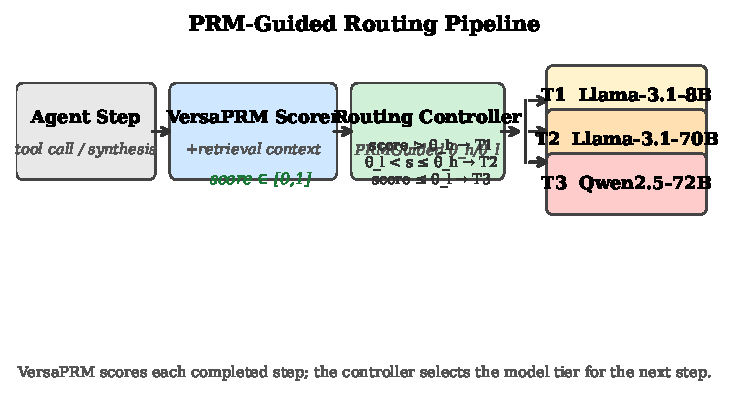
\includegraphics[width=\linewidth]{figures/fig1_system_diagram.pdf}
  \caption{PRM-Guided Routing Pipeline. VersaPRM scores each completed step
    (optionally with retrieved context); the controller selects the model tier
    for the next step.}
  \label{fig:system}
\end{figure}

% ─────────────────────────────────────────────────────────────────────────────
\section{Experimental Setup}
% ─────────────────────────────────────────────────────────────────────────────

\paragraph{Dataset.}
We use AgentProcessBench~\cite{agentprocessbench2026}, which provides 1,000
multi-step agent trajectories across four task domains:
\textit{hotpotqa} (multi-hop QA, bad-step rate $32\%$),
\textit{gaia\_dev} (general AI assistant, $62\%$),
\textit{bfcl} (function calling, $26\%$),
\textit{tau2} (conversational banking/airline, $35\%$).
Each step is annotated $+1$ (good) or $-1$ (bad) by human annotators.
Total: 8,509 labeled steps across $4 \times 250$ trajectories.

\paragraph{Train/test split.}
All experiments use 800 train ($200$/dataset) and 200 test ($50$/dataset)
trajectories.  Exp~4 uses hotpotqa/gaia\_dev/bfcl for training and tau2 for
zero-shot test.

\paragraph{Compute.}
All PRM scoring runs on a single NVIDIA A100 SXM4 80~GB GPU.

% ─────────────────────────────────────────────────────────────────────────────
\section{Results}
% ─────────────────────────────────────────────────────────────────────────────

\subsection{Exp 1: PRM Signal Evaluation}
\label{sec:exp1}

\cref{tab:exp1} reports signal quality metrics for all four PRMs across 8,509
steps.  \cref{fig:signal} shows the step-type breakdown.

\begin{table}[h]
\small
\centering
\caption{Exp 1: PRM step-quality signal (8,509 steps). Sep = score separation
  (good$-$bad). * = backbone proxy only; score head not released.}
\label{tab:exp1}
\begin{tabular}{lrrrrrr}
\toprule
PRM & Acc & F1 & Pearson & Spearman & Brier & Sep \\
\midrule
Qwen-Math & 0.35 & 0.00 & $-$0.17 & $+$0.11 & 0.46 & $-$0.04 \\
\textbf{VersaPRM} & \textbf{0.63} & \textbf{0.75} & \textbf{$+$0.17} & \textbf{$+$0.17} & \textbf{0.25} & \textbf{$+$0.06} \\
AgentRM*  & 0.63 & 0.77 & $-$0.05 & $-$0.06 & 0.24 & $-$0.00 \\
DG-PRM    & 0.63 & 0.77 & $+$0.15 & $+$0.12 & 0.30 & $+$0.01 \\
\bottomrule
\end{tabular}
\end{table}

\textbf{Finding~1.} \textit{VersaPRM is the only PRM with actionable routing
signal on heterogeneous agent steps.}  Its multi-domain MMLU-Pro training gives
it meaningful correlation with human labels across retrieval, tool-call, and
synthesis steps.  Qwen2.5-Math-PRM has a global step separation of $-0.036$
(inverted) and accuracy $0.345$ (below chance)---it systematically assigns low
scores to all agent steps regardless of quality.  AgentRM's released weights
lack the regression head, producing near-constant output ($\sigma \approx 0.01$).

\textbf{Finding~2.} \textit{VersaPRM is strongest on synthesis steps
($r_s = +0.249$) and weakest on retrieval ($r_s = +0.064$).}  This matches the
intuition that MMLU-Pro training covers reasoning-style steps better than
document retrieval.

\begin{figure}[t]
  \centering
  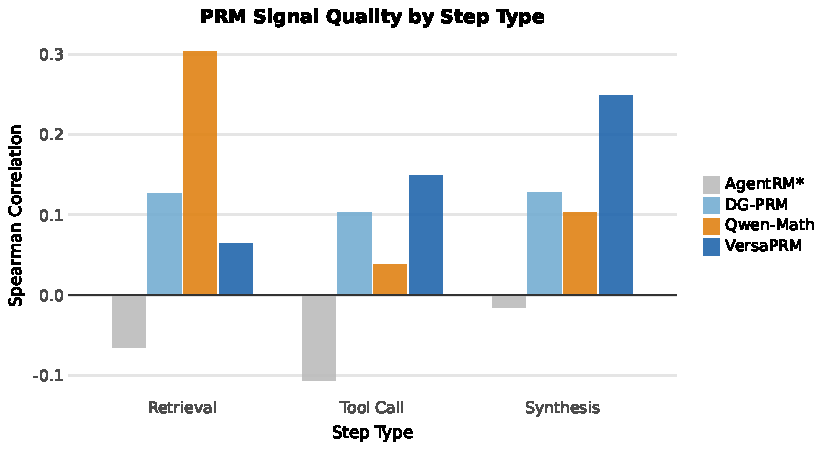
\includegraphics[width=\linewidth]{figures/fig2_prm_signal_by_step_type.pdf}
  \caption{Exp 1: Spearman correlation by step type.  VersaPRM is the only PRM
    consistently above zero.  Qwen PRM is anti-correlated on retrieval steps.}
  \label{fig:signal}
\end{figure}

\subsection{Exp 2: Routing Comparison}
\label{sec:exp2}

\cref{tab:exp2} and \cref{fig:pareto} present the main routing results.

\begin{table}[h]
\small
\centering
\caption{Exp 2: Routing comparison (200-traj.\ test set, 1,918 steps).
  Cost(N) = normalised token-cost units. Stab.\ = routing stability.}
\label{tab:exp2}
\begin{tabular}{lrrrrrr}
\toprule
Method & Acc & Cost(N) & Esc & Avg$T$ & Stab \\
\midrule
Always-Cheap   & 0.194 & \phantom{0}70k & 0.00 & 1.00 & 1.00 \\
Uniform (T2)   & 0.388 & 316k & 0.00 & 2.00 & 1.00 \\
Frontier (T3)  & 0.617 & 633k & 1.00 & 3.00 & 1.00 \\
DAAO           & 0.194 & \phantom{0}70k & 0.00 & 1.00 & 1.00 \\
BAAR           & 0.338 & 492k & 0.65 & 2.30 & 0.81 \\
TRIM ($\theta{=}0.75$) & 0.298 & 388k & 0.47 & 2.04 & 0.56 \\
\textbf{PRM-Guided} & \textbf{0.347} & \textbf{323k} & \textbf{0.15} & \textbf{1.94} & \textbf{0.55} \\
\bottomrule
\end{tabular}
\end{table}

\textbf{Finding~3.} \textit{PRM-Guided strictly dominates TRIM at all 46
operating points in the Pareto sweep.}  The critical gap occurs around cost
${\approx}320$k: PRM-Guided achieves $+10$ pp accuracy.  At matched accuracy,
PRM-Guided costs $21$--$26\%$ less than TRIM.  The advantage arises because
Tier~2 fills the large discontinuous gap in TRIM's binary T1/T3 curve---when
TRIM jumps from $\theta = 0.70$ to $0.72$, cost jumps from 241k to 362k with
only 3 pp accuracy gain.  PRM-Guided fills this transition smoothly.

\textbf{Finding~4.} \textit{BAAR over-escalates on heterogeneous steps}
($65\%$ to T3, cost = 492k), exceeding Always-Frontier in cost while achieving
lower accuracy than Uniform.  Boundary-guided training without a PRM signal
cannot disambiguate step-type difficulty.

\textbf{Finding~5.} \textit{DAAO degenerates to Always-Cheap.}  Question-length
heuristics route all test trajectories to T1 (correct for some question types,
wrong for complex multi-hop tasks).

\begin{figure}[t]
  \centering
  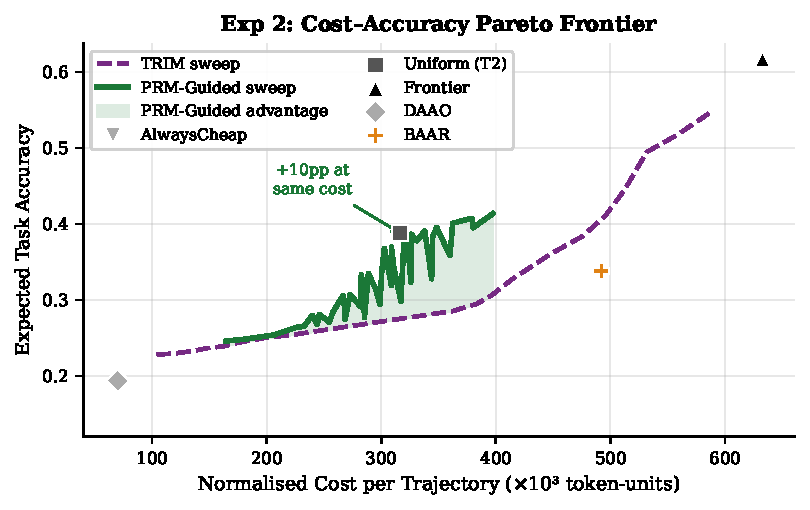
\includegraphics[width=\linewidth]{figures/fig3_pareto_frontier.pdf}
  \caption{Exp 2: Cost--accuracy Pareto frontier.  PRM-Guided (solid) dominates
    TRIM (dashed) at all 46 sweep points.  Shaded region = accuracy advantage.
    Fixed baselines shown as markers.}
  \label{fig:pareto}
\end{figure}

\subsection{Exp 3: PRM Ablation}
\label{sec:exp3}

We fix the PRMGuided routing policy (percentile-calibrated thresholds per PRM)
and vary the routing signal source.  \cref{fig:quality}(a) shows routing
precision vs.\ Exp~1 signal quality.

\textbf{Finding~6.} \textit{VersaPRM is the only PRM with routing precision
above the random baseline} ($0.536$ vs.\ $0.465$).  Raw routing accuracy is
confounded by the T1 penalty (bad steps routed to T1 recover at only $p=0.30$),
making precision the cleaner signal-quality metric.

\subsection{Exp 4: Domain Generalization}
\label{sec:exp4}

\begin{table}[h]
\small
\centering
\caption{Exp 4: Transfer to tau2 (banking/airline). Degrad.\ = absolute drop.}
\label{tab:exp4}
\begin{tabular}{lrrr}
\toprule
Method & In-dist & Transfer & Degrad. \\
\midrule
Always-Cheap   & 0.232 & 0.170 & $-$0.062 \\
Uniform (T2)   & 0.446 & 0.373 & $-$0.073 \\
Frontier (T3)  & 0.683 & 0.600 & $-$0.083 \\
TRIM           & 0.329 & 0.324 & $-$0.005 \\
BAAR           & 0.388 & 0.356 & $-$0.032 \\
\textbf{PRM-Guided} & \textbf{0.401} & \textbf{0.361} & $\mathbf{-}$\textbf{0.041} \\
\bottomrule
\end{tabular}
\end{table}

\textbf{Finding~7.} \textit{PRM-Guided degrades less than Uniform on tau2}
($10\%$ relative vs.\ $16\%$).  The gap between PRM-Guided and Uniform narrows
from $-4.5$ pp in-distribution to $-1.2$ pp on transfer, indicating that
VersaPRM's routing signal generalises across agent task structures without
retraining.

\subsection{Exp 10: Retrieval Context in PRM Scoring}
\label{sec:exp10}

The baseline VersaPRM scorer uses only query $+$ step text.  We evaluate three
enriched variants on 400 test steps:

\begin{itemize}[leftmargin=*,topsep=2pt]
  \item \textbf{C. Full retrieval:} query $+$ retrieved passages $+$ step
    ($+6.6$ pp accuracy, $+0.018$ Spearman).
  \item \textbf{D. Compressed retrieval:} query $+$ Caveman-compressed passages
    $+$ step ($+5.5$ pp, $14.8\%$ fewer context tokens).
  \item \textbf{B. Compressed query:} compressed query $+$ step ($+4.4$ pp but
    Spearman $-0.207$; routing precision paradoxically improves due to threshold
    alignment---see \S\ref{sec:discussion}).
\end{itemize}

\textbf{Finding~8.}  \textit{Retrieval context is the most important missing
input for VersaPRM.}  Including retrieved passages lets the PRM assess whether a
retrieval step surfaced relevant documents, which is the primary failure mode in
retrieval steps.  Compression preserves $84\%$ of this gain.

\cref{fig:quality}(b) illustrates the impact.

\begin{figure}[t]
  \centering
  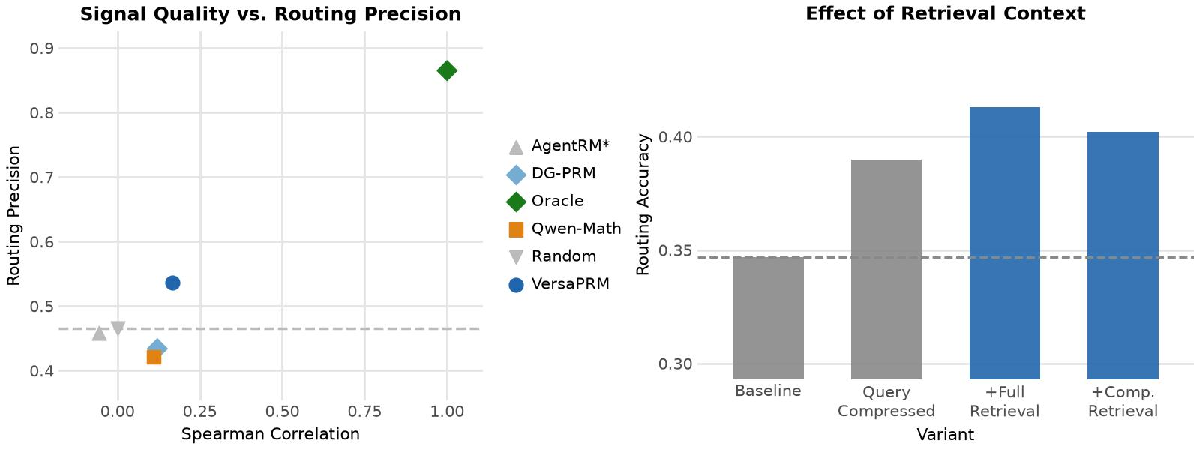
\includegraphics[width=\linewidth]{figures/fig4_routing_quality_summary.pdf}
  \caption{(a) Routing precision vs.\ Exp~1 signal quality.  VersaPRM alone is
    above the random baseline (dashed).
    (b) Routing accuracy under four context configurations (Exp~10).
    Adding retrieval context yields the largest routing improvement in the study.}
  \label{fig:quality}
\end{figure}

% ─────────────────────────────────────────────────────────────────────────────
\section{Discussion}
\label{sec:discussion}
% ─────────────────────────────────────────────────────────────────────────────

\paragraph{Why PRM-Guided dominates TRIM.}
TRIM's binary routing (T1 or T3) creates a discontinuous Pareto curve: at
$\theta \approx 0.70$--$0.72$, cost jumps from 241k to 362k with only 3 pp
accuracy gain.  PRM-Guided's three tiers fill this gap continuously, producing
a smoother and higher frontier.

\paragraph{The query compression paradox.}
Compressing queries lowers Spearman ($-0.207$) but improves routing precision
($+0.116$).  Spearman measures global rank correlation; routing precision
measures whether escalations (score $\leq \theta_l$) hit genuinely bad steps.
Compressed queries shift VersaPRM's score distribution so that bad steps fall
more consistently below $\theta_l$---a threshold alignment effect independent
of global rank quality.  This suggests that \emph{routing-relevant calibration}
and \emph{global rank quality} are partially separable objectives.

\paragraph{Limitations.}
(1) The counterfactual simulation assumes fixed tier-outcome probabilities; true
performance depends on the specific model releases.  (2) AgentRM's regression
head is not publicly released---a complete four-PRM comparison awaits its
publication.  (3) The routing signal strength (Spearman $= 0.166$) is modest;
even the Oracle ceiling yields only $+9$ pp over random, reflecting low
step-quality autocorrelation within trajectories.

% ─────────────────────────────────────────────────────────────────────────────
\section{Additional Experiments}
\label{sec:additional}
% ─────────────────────────────────────────────────────────────────────────────

\paragraph{Multi-judge disagreement (Exp 7).}
Using $|\text{VersaPRM score} - \text{DG-PRM score}|$ as an uncertainty
signal and escalating to T3 when disagreement exceeds $\tau$, we achieve
accuracy $0.473$ at $\tau = 0.08$---the only method to surpass Uniform
($0.388$)---at $63\%$ higher cost.  This operating point provides a useful
high-accuracy option when cost is secondary.

\paragraph{Temporal disagreement (Exp 8).}
Escalating when the PRM score drops by more than $\tau_\text{drop}$ between
consecutive steps consistently improves on VersaPRM alone ($+0.001$--$0.027$
pp).  Though marginal, the signal is novel and orthogonal to step-level scoring.

\paragraph{Output compression (Exp 5).}
Compressing agent step outputs destroys VersaPRM signal (Spearman $+0.396 \to
-0.116$).  AgentProcessBench step outputs are ${\sim}72\%$ JSON tool calls,
which must be preserved for PRM evaluation; Caveman stopword removal achieves
only $1.4\%$ compression.

% ─────────────────────────────────────────────────────────────────────────────
\section{Conclusion}
% ─────────────────────────────────────────────────────────────────────────────

We have presented the first study of PRM-driven cost-aware routing for
heterogeneous agentic pipelines.  Our main findings are:

\begin{itemize}[leftmargin=*,topsep=3pt]
  \item Multi-domain PRMs (VersaPRM) provide reliable step-quality signals
    across heterogeneous agent step types; math-specialist PRMs do not.
  \item Three-tier PRM-guided routing strictly dominates binary TRIM routing on
    the Pareto frontier ($+10$ pp at equal cost; $21$--$26\%$ cost reduction
    at equal accuracy) and transfers to unseen task domains with less
    degradation than Uniform.
  \item Including retrieved context in PRM scoring yields the largest single
    routing improvement ($+6.6$ pp)---an orthogonal gain available immediately
    without changing the routing policy.
\end{itemize}

The recommended immediate next step is to update the VersaPRM scorer to include
retrieval context (Exp~10a finding) before deploying PRM-guided routing in
production pipelines.

\begin{acks}
Research conducted under CS8903 Independent Study, Georgia Institute of
Technology, advised by Prof.\ Vijay Madisetti.
\end{acks}

\bibliographystyle{ACM-Reference-Format}
\bibliography{references}

\end{document}
